% Graphic for TeX using PGF
% Title: /home/satenske/cours/AP/obj3/uml19.dia
% Creator: Dia v0.97.1
% CreationDate: Thu Sep 22 10:27:24 2011
% For: satenske
% \usepackage{tikz}
% The following commands are not supported in PSTricks at present
% We define them conditionally, so when they are implemented,
% this pgf file will use them.
\ifx\du\undefined
  \newlength{\du}
\fi
\setlength{\du}{15\unitlength}
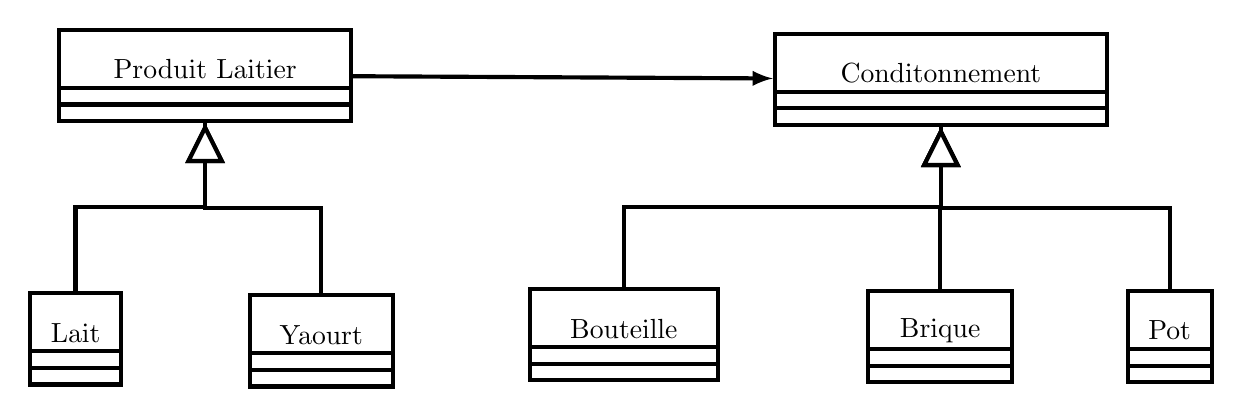
\begin{tikzpicture}
\pgftransformxscale{1.000000}
\pgftransformyscale{-1.000000}
\definecolor{dialinecolor}{rgb}{0.000000, 0.000000, 0.000000}
\pgfsetstrokecolor{dialinecolor}
\definecolor{dialinecolor}{rgb}{1.000000, 1.000000, 1.000000}
\pgfsetfillcolor{dialinecolor}
\pgfsetlinewidth{0.100000\du}
\pgfsetdash{}{0pt}
\definecolor{dialinecolor}{rgb}{1.000000, 1.000000, 1.000000}
\pgfsetfillcolor{dialinecolor}
\fill (7.525000\du,4.865000\du)--(7.525000\du,6.265000\du)--(14.555000\du,6.265000\du)--(14.555000\du,4.865000\du)--cycle;
\definecolor{dialinecolor}{rgb}{0.000000, 0.000000, 0.000000}
\pgfsetstrokecolor{dialinecolor}
\draw (7.525000\du,4.865000\du)--(7.525000\du,6.265000\du)--(14.555000\du,6.265000\du)--(14.555000\du,4.865000\du)--cycle;
% setfont left to latex
\definecolor{dialinecolor}{rgb}{0.000000, 0.000000, 0.000000}
\pgfsetstrokecolor{dialinecolor}
\node at (11.040000\du,5.815000\du){Produit Laitier};
\definecolor{dialinecolor}{rgb}{1.000000, 1.000000, 1.000000}
\pgfsetfillcolor{dialinecolor}
\fill (7.525000\du,6.265000\du)--(7.525000\du,6.665000\du)--(14.555000\du,6.665000\du)--(14.555000\du,6.265000\du)--cycle;
\definecolor{dialinecolor}{rgb}{0.000000, 0.000000, 0.000000}
\pgfsetstrokecolor{dialinecolor}
\draw (7.525000\du,6.265000\du)--(7.525000\du,6.665000\du)--(14.555000\du,6.665000\du)--(14.555000\du,6.265000\du)--cycle;
\definecolor{dialinecolor}{rgb}{1.000000, 1.000000, 1.000000}
\pgfsetfillcolor{dialinecolor}
\fill (7.525000\du,6.665000\du)--(7.525000\du,7.065000\du)--(14.555000\du,7.065000\du)--(14.555000\du,6.665000\du)--cycle;
\definecolor{dialinecolor}{rgb}{0.000000, 0.000000, 0.000000}
\pgfsetstrokecolor{dialinecolor}
\draw (7.525000\du,6.665000\du)--(7.525000\du,7.065000\du)--(14.555000\du,7.065000\du)--(14.555000\du,6.665000\du)--cycle;
\pgfsetlinewidth{0.100000\du}
\pgfsetdash{}{0pt}
\definecolor{dialinecolor}{rgb}{1.000000, 1.000000, 1.000000}
\pgfsetfillcolor{dialinecolor}
\fill (6.815000\du,11.210000\du)--(6.815000\du,12.610000\du)--(9.022500\du,12.610000\du)--(9.022500\du,11.210000\du)--cycle;
\definecolor{dialinecolor}{rgb}{0.000000, 0.000000, 0.000000}
\pgfsetstrokecolor{dialinecolor}
\draw (6.815000\du,11.210000\du)--(6.815000\du,12.610000\du)--(9.022500\du,12.610000\du)--(9.022500\du,11.210000\du)--cycle;
% setfont left to latex
\definecolor{dialinecolor}{rgb}{0.000000, 0.000000, 0.000000}
\pgfsetstrokecolor{dialinecolor}
\node at (7.918750\du,12.160000\du){Lait};
\definecolor{dialinecolor}{rgb}{1.000000, 1.000000, 1.000000}
\pgfsetfillcolor{dialinecolor}
\fill (6.815000\du,12.610000\du)--(6.815000\du,13.010000\du)--(9.022500\du,13.010000\du)--(9.022500\du,12.610000\du)--cycle;
\definecolor{dialinecolor}{rgb}{0.000000, 0.000000, 0.000000}
\pgfsetstrokecolor{dialinecolor}
\draw (6.815000\du,12.610000\du)--(6.815000\du,13.010000\du)--(9.022500\du,13.010000\du)--(9.022500\du,12.610000\du)--cycle;
\definecolor{dialinecolor}{rgb}{1.000000, 1.000000, 1.000000}
\pgfsetfillcolor{dialinecolor}
\fill (6.815000\du,13.010000\du)--(6.815000\du,13.410000\du)--(9.022500\du,13.410000\du)--(9.022500\du,13.010000\du)--cycle;
\definecolor{dialinecolor}{rgb}{0.000000, 0.000000, 0.000000}
\pgfsetstrokecolor{dialinecolor}
\draw (6.815000\du,13.010000\du)--(6.815000\du,13.410000\du)--(9.022500\du,13.410000\du)--(9.022500\du,13.010000\du)--cycle;
\pgfsetlinewidth{0.100000\du}
\pgfsetdash{}{0pt}
\definecolor{dialinecolor}{rgb}{1.000000, 1.000000, 1.000000}
\pgfsetfillcolor{dialinecolor}
\fill (12.115000\du,11.260000\du)--(12.115000\du,12.660000\du)--(15.560000\du,12.660000\du)--(15.560000\du,11.260000\du)--cycle;
\definecolor{dialinecolor}{rgb}{0.000000, 0.000000, 0.000000}
\pgfsetstrokecolor{dialinecolor}
\draw (12.115000\du,11.260000\du)--(12.115000\du,12.660000\du)--(15.560000\du,12.660000\du)--(15.560000\du,11.260000\du)--cycle;
% setfont left to latex
\definecolor{dialinecolor}{rgb}{0.000000, 0.000000, 0.000000}
\pgfsetstrokecolor{dialinecolor}
\node at (13.837500\du,12.210000\du){Yaourt};
\definecolor{dialinecolor}{rgb}{1.000000, 1.000000, 1.000000}
\pgfsetfillcolor{dialinecolor}
\fill (12.115000\du,12.660000\du)--(12.115000\du,13.060000\du)--(15.560000\du,13.060000\du)--(15.560000\du,12.660000\du)--cycle;
\definecolor{dialinecolor}{rgb}{0.000000, 0.000000, 0.000000}
\pgfsetstrokecolor{dialinecolor}
\draw (12.115000\du,12.660000\du)--(12.115000\du,13.060000\du)--(15.560000\du,13.060000\du)--(15.560000\du,12.660000\du)--cycle;
\definecolor{dialinecolor}{rgb}{1.000000, 1.000000, 1.000000}
\pgfsetfillcolor{dialinecolor}
\fill (12.115000\du,13.060000\du)--(12.115000\du,13.460000\du)--(15.560000\du,13.460000\du)--(15.560000\du,13.060000\du)--cycle;
\definecolor{dialinecolor}{rgb}{0.000000, 0.000000, 0.000000}
\pgfsetstrokecolor{dialinecolor}
\draw (12.115000\du,13.060000\du)--(12.115000\du,13.460000\du)--(15.560000\du,13.460000\du)--(15.560000\du,13.060000\du)--cycle;
\pgfsetlinewidth{0.100000\du}
\pgfsetdash{}{0pt}
\definecolor{dialinecolor}{rgb}{1.000000, 1.000000, 1.000000}
\pgfsetfillcolor{dialinecolor}
\fill (18.865000\du,11.110000\du)--(18.865000\du,12.510000\du)--(23.387500\du,12.510000\du)--(23.387500\du,11.110000\du)--cycle;
\definecolor{dialinecolor}{rgb}{0.000000, 0.000000, 0.000000}
\pgfsetstrokecolor{dialinecolor}
\draw (18.865000\du,11.110000\du)--(18.865000\du,12.510000\du)--(23.387500\du,12.510000\du)--(23.387500\du,11.110000\du)--cycle;
% setfont left to latex
\definecolor{dialinecolor}{rgb}{0.000000, 0.000000, 0.000000}
\pgfsetstrokecolor{dialinecolor}
\node at (21.126250\du,12.060000\du){Bouteille};
\definecolor{dialinecolor}{rgb}{1.000000, 1.000000, 1.000000}
\pgfsetfillcolor{dialinecolor}
\fill (18.865000\du,12.510000\du)--(18.865000\du,12.910000\du)--(23.387500\du,12.910000\du)--(23.387500\du,12.510000\du)--cycle;
\definecolor{dialinecolor}{rgb}{0.000000, 0.000000, 0.000000}
\pgfsetstrokecolor{dialinecolor}
\draw (18.865000\du,12.510000\du)--(18.865000\du,12.910000\du)--(23.387500\du,12.910000\du)--(23.387500\du,12.510000\du)--cycle;
\definecolor{dialinecolor}{rgb}{1.000000, 1.000000, 1.000000}
\pgfsetfillcolor{dialinecolor}
\fill (18.865000\du,12.910000\du)--(18.865000\du,13.310000\du)--(23.387500\du,13.310000\du)--(23.387500\du,12.910000\du)--cycle;
\definecolor{dialinecolor}{rgb}{0.000000, 0.000000, 0.000000}
\pgfsetstrokecolor{dialinecolor}
\draw (18.865000\du,12.910000\du)--(18.865000\du,13.310000\du)--(23.387500\du,13.310000\du)--(23.387500\du,12.910000\du)--cycle;
\pgfsetlinewidth{0.100000\du}
\pgfsetdash{}{0pt}
\definecolor{dialinecolor}{rgb}{1.000000, 1.000000, 1.000000}
\pgfsetfillcolor{dialinecolor}
\fill (27.015000\du,11.160000\du)--(27.015000\du,12.560000\du)--(30.480000\du,12.560000\du)--(30.480000\du,11.160000\du)--cycle;
\definecolor{dialinecolor}{rgb}{0.000000, 0.000000, 0.000000}
\pgfsetstrokecolor{dialinecolor}
\draw (27.015000\du,11.160000\du)--(27.015000\du,12.560000\du)--(30.480000\du,12.560000\du)--(30.480000\du,11.160000\du)--cycle;
% setfont left to latex
\definecolor{dialinecolor}{rgb}{0.000000, 0.000000, 0.000000}
\pgfsetstrokecolor{dialinecolor}
\node at (28.747500\du,12.110000\du){Brique};
\definecolor{dialinecolor}{rgb}{1.000000, 1.000000, 1.000000}
\pgfsetfillcolor{dialinecolor}
\fill (27.015000\du,12.560000\du)--(27.015000\du,12.960000\du)--(30.480000\du,12.960000\du)--(30.480000\du,12.560000\du)--cycle;
\definecolor{dialinecolor}{rgb}{0.000000, 0.000000, 0.000000}
\pgfsetstrokecolor{dialinecolor}
\draw (27.015000\du,12.560000\du)--(27.015000\du,12.960000\du)--(30.480000\du,12.960000\du)--(30.480000\du,12.560000\du)--cycle;
\definecolor{dialinecolor}{rgb}{1.000000, 1.000000, 1.000000}
\pgfsetfillcolor{dialinecolor}
\fill (27.015000\du,12.960000\du)--(27.015000\du,13.360000\du)--(30.480000\du,13.360000\du)--(30.480000\du,12.960000\du)--cycle;
\definecolor{dialinecolor}{rgb}{0.000000, 0.000000, 0.000000}
\pgfsetstrokecolor{dialinecolor}
\draw (27.015000\du,12.960000\du)--(27.015000\du,13.360000\du)--(30.480000\du,13.360000\du)--(30.480000\du,12.960000\du)--cycle;
\pgfsetlinewidth{0.100000\du}
\pgfsetdash{}{0pt}
\definecolor{dialinecolor}{rgb}{1.000000, 1.000000, 1.000000}
\pgfsetfillcolor{dialinecolor}
\fill (33.265000\du,11.160000\du)--(33.265000\du,12.560000\du)--(35.285000\du,12.560000\du)--(35.285000\du,11.160000\du)--cycle;
\definecolor{dialinecolor}{rgb}{0.000000, 0.000000, 0.000000}
\pgfsetstrokecolor{dialinecolor}
\draw (33.265000\du,11.160000\du)--(33.265000\du,12.560000\du)--(35.285000\du,12.560000\du)--(35.285000\du,11.160000\du)--cycle;
% setfont left to latex
\definecolor{dialinecolor}{rgb}{0.000000, 0.000000, 0.000000}
\pgfsetstrokecolor{dialinecolor}
\node at (34.275000\du,12.110000\du){Pot};
\definecolor{dialinecolor}{rgb}{1.000000, 1.000000, 1.000000}
\pgfsetfillcolor{dialinecolor}
\fill (33.265000\du,12.560000\du)--(33.265000\du,12.960000\du)--(35.285000\du,12.960000\du)--(35.285000\du,12.560000\du)--cycle;
\definecolor{dialinecolor}{rgb}{0.000000, 0.000000, 0.000000}
\pgfsetstrokecolor{dialinecolor}
\draw (33.265000\du,12.560000\du)--(33.265000\du,12.960000\du)--(35.285000\du,12.960000\du)--(35.285000\du,12.560000\du)--cycle;
\definecolor{dialinecolor}{rgb}{1.000000, 1.000000, 1.000000}
\pgfsetfillcolor{dialinecolor}
\fill (33.265000\du,12.960000\du)--(33.265000\du,13.360000\du)--(35.285000\du,13.360000\du)--(35.285000\du,12.960000\du)--cycle;
\definecolor{dialinecolor}{rgb}{0.000000, 0.000000, 0.000000}
\pgfsetstrokecolor{dialinecolor}
\draw (33.265000\du,12.960000\du)--(33.265000\du,13.360000\du)--(35.285000\du,13.360000\du)--(35.285000\du,12.960000\du)--cycle;
\pgfsetlinewidth{0.100000\du}
\pgfsetdash{}{0pt}
\definecolor{dialinecolor}{rgb}{1.000000, 1.000000, 1.000000}
\pgfsetfillcolor{dialinecolor}
\fill (24.765000\du,4.960000\du)--(24.765000\du,6.360000\du)--(32.762500\du,6.360000\du)--(32.762500\du,4.960000\du)--cycle;
\definecolor{dialinecolor}{rgb}{0.000000, 0.000000, 0.000000}
\pgfsetstrokecolor{dialinecolor}
\draw (24.765000\du,4.960000\du)--(24.765000\du,6.360000\du)--(32.762500\du,6.360000\du)--(32.762500\du,4.960000\du)--cycle;
% setfont left to latex
\definecolor{dialinecolor}{rgb}{0.000000, 0.000000, 0.000000}
\pgfsetstrokecolor{dialinecolor}
\node at (28.763750\du,5.910000\du){Conditonnement};
\definecolor{dialinecolor}{rgb}{1.000000, 1.000000, 1.000000}
\pgfsetfillcolor{dialinecolor}
\fill (24.765000\du,6.360000\du)--(24.765000\du,6.760000\du)--(32.762500\du,6.760000\du)--(32.762500\du,6.360000\du)--cycle;
\definecolor{dialinecolor}{rgb}{0.000000, 0.000000, 0.000000}
\pgfsetstrokecolor{dialinecolor}
\draw (24.765000\du,6.360000\du)--(24.765000\du,6.760000\du)--(32.762500\du,6.760000\du)--(32.762500\du,6.360000\du)--cycle;
\definecolor{dialinecolor}{rgb}{1.000000, 1.000000, 1.000000}
\pgfsetfillcolor{dialinecolor}
\fill (24.765000\du,6.760000\du)--(24.765000\du,7.160000\du)--(32.762500\du,7.160000\du)--(32.762500\du,6.760000\du)--cycle;
\definecolor{dialinecolor}{rgb}{0.000000, 0.000000, 0.000000}
\pgfsetstrokecolor{dialinecolor}
\draw (24.765000\du,6.760000\du)--(24.765000\du,7.160000\du)--(32.762500\du,7.160000\du)--(32.762500\du,6.760000\du)--cycle;
\pgfsetlinewidth{0.100000\du}
\pgfsetdash{}{0pt}
\pgfsetmiterjoin
\pgfsetbuttcap
{
\definecolor{dialinecolor}{rgb}{0.000000, 0.000000, 0.000000}
\pgfsetfillcolor{dialinecolor}
% was here!!!
\definecolor{dialinecolor}{rgb}{0.000000, 0.000000, 0.000000}
\pgfsetstrokecolor{dialinecolor}
\draw (11.040000\du,7.115281\du)--(11.040000\du,9.137500\du)--(7.918750\du,9.137500\du)--(7.918750\du,11.159719\du);
}
\definecolor{dialinecolor}{rgb}{0.000000, 0.000000, 0.000000}
\pgfsetstrokecolor{dialinecolor}
\draw (11.040000\du,8.027084\du)--(11.040000\du,9.137500\du)--(7.918750\du,9.137500\du)--(7.918750\du,11.159719\du);
\pgfsetmiterjoin
\definecolor{dialinecolor}{rgb}{1.000000, 1.000000, 1.000000}
\pgfsetfillcolor{dialinecolor}
\fill (11.440000\du,8.027084\du)--(11.040000\du,7.227084\du)--(10.640000\du,8.027084\du)--cycle;
\pgfsetlinewidth{0.100000\du}
\pgfsetdash{}{0pt}
\pgfsetmiterjoin
\definecolor{dialinecolor}{rgb}{0.000000, 0.000000, 0.000000}
\pgfsetstrokecolor{dialinecolor}
\draw (11.440000\du,8.027084\du)--(11.040000\du,7.227084\du)--(10.640000\du,8.027084\du)--cycle;
% setfont left to latex
\pgfsetlinewidth{0.100000\du}
\pgfsetdash{}{0pt}
\pgfsetmiterjoin
\pgfsetbuttcap
{
\definecolor{dialinecolor}{rgb}{0.000000, 0.000000, 0.000000}
\pgfsetfillcolor{dialinecolor}
% was here!!!
\definecolor{dialinecolor}{rgb}{0.000000, 0.000000, 0.000000}
\pgfsetstrokecolor{dialinecolor}
\draw (11.040000\du,7.115281\du)--(11.040000\du,9.162500\du)--(13.837500\du,9.162500\du)--(13.837500\du,11.209719\du);
}
\definecolor{dialinecolor}{rgb}{0.000000, 0.000000, 0.000000}
\pgfsetstrokecolor{dialinecolor}
\draw (11.040000\du,8.027084\du)--(11.040000\du,9.162500\du)--(13.837500\du,9.162500\du)--(13.837500\du,11.209719\du);
\pgfsetmiterjoin
\definecolor{dialinecolor}{rgb}{1.000000, 1.000000, 1.000000}
\pgfsetfillcolor{dialinecolor}
\fill (11.440000\du,8.027084\du)--(11.040000\du,7.227084\du)--(10.640000\du,8.027084\du)--cycle;
\pgfsetlinewidth{0.100000\du}
\pgfsetdash{}{0pt}
\pgfsetmiterjoin
\definecolor{dialinecolor}{rgb}{0.000000, 0.000000, 0.000000}
\pgfsetstrokecolor{dialinecolor}
\draw (11.440000\du,8.027084\du)--(11.040000\du,7.227084\du)--(10.640000\du,8.027084\du)--cycle;
% setfont left to latex
\pgfsetlinewidth{0.100000\du}
\pgfsetdash{}{0pt}
\pgfsetmiterjoin
\pgfsetbuttcap
{
\definecolor{dialinecolor}{rgb}{0.000000, 0.000000, 0.000000}
\pgfsetfillcolor{dialinecolor}
% was here!!!
\definecolor{dialinecolor}{rgb}{0.000000, 0.000000, 0.000000}
\pgfsetstrokecolor{dialinecolor}
\draw (28.763750\du,7.210281\du)--(28.763750\du,9.135000\du)--(21.126250\du,9.135000\du)--(21.126250\du,11.059719\du);
}
\definecolor{dialinecolor}{rgb}{0.000000, 0.000000, 0.000000}
\pgfsetstrokecolor{dialinecolor}
\draw (28.763750\du,8.122084\du)--(28.763750\du,9.135000\du)--(21.126250\du,9.135000\du)--(21.126250\du,11.059719\du);
\pgfsetmiterjoin
\definecolor{dialinecolor}{rgb}{1.000000, 1.000000, 1.000000}
\pgfsetfillcolor{dialinecolor}
\fill (29.163750\du,8.122084\du)--(28.763750\du,7.322084\du)--(28.363750\du,8.122084\du)--cycle;
\pgfsetlinewidth{0.100000\du}
\pgfsetdash{}{0pt}
\pgfsetmiterjoin
\definecolor{dialinecolor}{rgb}{0.000000, 0.000000, 0.000000}
\pgfsetstrokecolor{dialinecolor}
\draw (29.163750\du,8.122084\du)--(28.763750\du,7.322084\du)--(28.363750\du,8.122084\du)--cycle;
% setfont left to latex
\pgfsetlinewidth{0.100000\du}
\pgfsetdash{}{0pt}
\pgfsetmiterjoin
\pgfsetbuttcap
{
\definecolor{dialinecolor}{rgb}{0.000000, 0.000000, 0.000000}
\pgfsetfillcolor{dialinecolor}
% was here!!!
\definecolor{dialinecolor}{rgb}{0.000000, 0.000000, 0.000000}
\pgfsetstrokecolor{dialinecolor}
\draw (28.763750\du,7.210281\du)--(28.763750\du,9.160000\du)--(28.747500\du,9.160000\du)--(28.747500\du,11.109719\du);
}
\definecolor{dialinecolor}{rgb}{0.000000, 0.000000, 0.000000}
\pgfsetstrokecolor{dialinecolor}
\draw (28.763750\du,8.122084\du)--(28.763750\du,9.160000\du)--(28.747500\du,9.160000\du)--(28.747500\du,11.109719\du);
\pgfsetmiterjoin
\definecolor{dialinecolor}{rgb}{1.000000, 1.000000, 1.000000}
\pgfsetfillcolor{dialinecolor}
\fill (29.163750\du,8.122084\du)--(28.763750\du,7.322084\du)--(28.363750\du,8.122084\du)--cycle;
\pgfsetlinewidth{0.100000\du}
\pgfsetdash{}{0pt}
\pgfsetmiterjoin
\definecolor{dialinecolor}{rgb}{0.000000, 0.000000, 0.000000}
\pgfsetstrokecolor{dialinecolor}
\draw (29.163750\du,8.122084\du)--(28.763750\du,7.322084\du)--(28.363750\du,8.122084\du)--cycle;
% setfont left to latex
\pgfsetlinewidth{0.100000\du}
\pgfsetdash{}{0pt}
\pgfsetmiterjoin
\pgfsetbuttcap
{
\definecolor{dialinecolor}{rgb}{0.000000, 0.000000, 0.000000}
\pgfsetfillcolor{dialinecolor}
% was here!!!
\definecolor{dialinecolor}{rgb}{0.000000, 0.000000, 0.000000}
\pgfsetstrokecolor{dialinecolor}
\draw (28.763750\du,7.210281\du)--(28.763750\du,9.160000\du)--(34.275000\du,9.160000\du)--(34.275000\du,11.109719\du);
}
\definecolor{dialinecolor}{rgb}{0.000000, 0.000000, 0.000000}
\pgfsetstrokecolor{dialinecolor}
\draw (28.763750\du,8.122084\du)--(28.763750\du,9.160000\du)--(34.275000\du,9.160000\du)--(34.275000\du,11.109719\du);
\pgfsetmiterjoin
\definecolor{dialinecolor}{rgb}{1.000000, 1.000000, 1.000000}
\pgfsetfillcolor{dialinecolor}
\fill (29.163750\du,8.122084\du)--(28.763750\du,7.322084\du)--(28.363750\du,8.122084\du)--cycle;
\pgfsetlinewidth{0.100000\du}
\pgfsetdash{}{0pt}
\pgfsetmiterjoin
\definecolor{dialinecolor}{rgb}{0.000000, 0.000000, 0.000000}
\pgfsetstrokecolor{dialinecolor}
\draw (29.163750\du,8.122084\du)--(28.763750\du,7.322084\du)--(28.363750\du,8.122084\du)--cycle;
% setfont left to latex
\pgfsetlinewidth{0.100000\du}
\pgfsetbuttcap
\pgfsetdash{}{0pt}
{
\definecolor{dialinecolor}{rgb}{0.000000, 0.000000, 0.000000}
\pgfsetfillcolor{dialinecolor}
% was here!!!
\pgfsetarrowsstart{latex}
\definecolor{dialinecolor}{rgb}{0.000000, 0.000000, 0.000000}
\pgfsetstrokecolor{dialinecolor}
\draw (24.715219\du,6.038300\du)--(14.588212\du,5.984019\du);
}
% setfont left to latex
\end{tikzpicture}
